% !TEX root = ../../../main.tex
% 来源：高中物理甲种本·第一册（力学）
% 章节：力 / 同一直线上的矢量的运算
% 原始文件：1.tex，行 1852-1867
% 类型：tikz
% ---
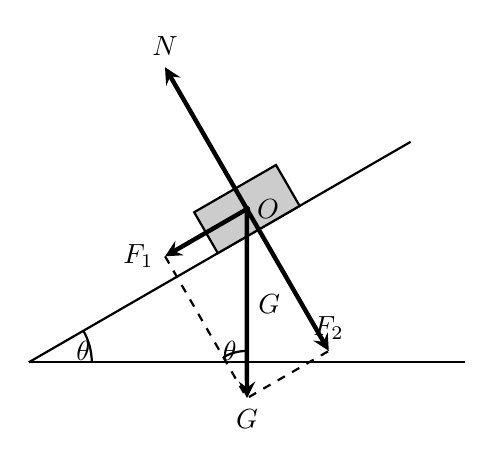
\begin{tikzpicture}[>=stealth,  thick, scale=.8]
\draw (0,0) --(6.93,0) ;
\draw (0,0)--(30:7);
\draw [rotate=30, fill=black!20] (6.93/2,0) rectangle (6.93/2+1.5,0+.75);
\draw [rotate=30, ->, ultra thick] (6.93/2+.75,.75/2)-- (6.93/2+.75,.75/2-2.6) node [above]{$F_2$};
\draw [rotate=30, ->, ultra thick] (6.93/2+.75,.75/2)-- (6.93/2+.75,.75/2+2.6) node [above]{$N$};
\draw [rotate=30, ->, ultra thick] (6.93/2+.75,.75/2)-- (6.93/2+.75-1.5,.75/2)node [left]{$F_1$};
\draw [rotate=30, ->, ultra thick] (6.93/2+.75,.75/2)--node [right]{$G$} (6.93/2+.75-1.5,.75/2-2.6)node [below]{$G$};
\draw [rotate=30, dashed] (6.93/2+.75-1.5,.75/2)--(6.93/2+.75-1.5,.75/2-2.6)-- (6.93/2+.75,.75/2-2.6);
\fill [rotate=30] (6.93/2+.75,.75/2) circle[radius=1.5pt] node [right]{$O$};

\draw [rotate=30](6.93/2+.75-1.5,.75/2-2.6+.75) arc(90:60:.75)node [left]{$\theta$};

\draw (0+1, 0) arc(0:30:1)node [below]{$\theta$};

\end{tikzpicture}
